\documentclass[main.tex]{subfiles}
%物体的运动
\begin{document}
\subsection{物体的运动}
\begin{definition}[世界运动]
一组两两不相交的世界线的集合$\psi$称为一个世界运动。
\end{definition}

一个世界运动中的世界线两两不相交是经典力学中的要求,称为“信息守恒定律”。通俗地说,任一时刻,某当前状态不可能有多于一种过去状态,也不可能有多于一种未来状态。

\begin{definition}[物体]
一个物体是一个非空集合$\mathcal{B}$,其元素$X\in\mathcal{B}$称为物质点。
\end{definition}

\begin{figure}[h]
\centering
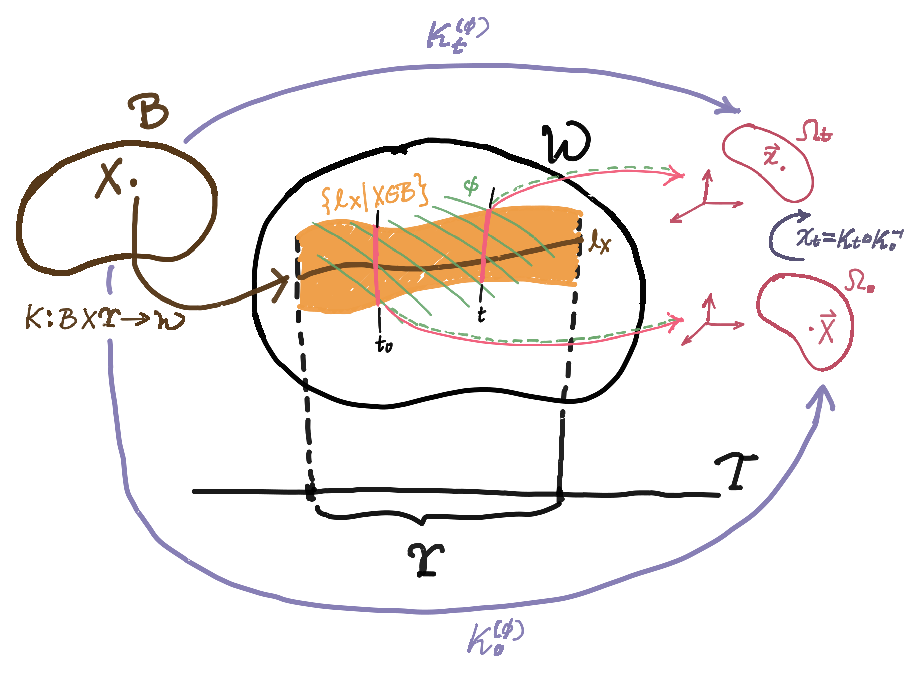
\includegraphics[width=0.5\textwidth]{images/III.2.1.eps}
\caption{物体的运动、运动学过程、放置、构型}
\label{fig:III.2.1}
\end{figure}

\begin{definition}[运动学过程、物体的运动]
如图\ref{fig:III.2.1}所示,设$\mathcal{B}$是一个物体,$\mathcal{W}$是事件世界,$\Upsilon$是时间$\mathcal{T}$的一个连通子集。映射$k:\mathcal{B}\times\Upsilon\rightarrow\mathcal{W}$称为一个运动学过程。对某物质点$X\in\mathcal{B}$,事件$k\left(X,a\right)=I_a,a\in\Upsilon$称$X$在时刻$a$经历的事件。集合$\left\{k\left(X,a\right)|a\in\Upsilon\right\}$是一条世界线的子集,记为$l_X$,称为物质点$X$的运动。$\mathcal{B}$的所有物质点的同一运动学过程$\left\{l_X|X\in\mathcal{B}\right\}$是一个世界运动的子集,记为$\psi_\mathcal{B}$,称为物体$\mathcal{B}$的运动。
\end{definition}

作为世界运动的子集,物体的运动中各物质点的运动也是两两不相交的。

我们考虑物体$\mathcal{B}$的一个物质点$X\in\mathcal{B}$在一段时间$\Upsilon$内的运动$l_X$。给定事件世界的标架$\phi$,则$l_X$的每个事件$l_X\left(a\right),a\in\Upsilon$,都必属于$\phi$的一条世界线$l_\phi\left(l_X\left(a\right)\right)$。该物质点在某时刻$a\in\Upsilon$的速度是如下导数
\[\left.\frac{d l_X\left(t\right)}{dt}\right|_{t=a}\equiv\lim_{s\to 0}\frac{l_\phi\left(l_X\left(a+s\right)\right)-l_\phi\left(l_X\left(a\right)\right)}{s},s\in\mathbb{R}
\]
同理可给出物质点$X$在时刻$a$的加速度。速度和加速度都是$\mathcal{V}_\phi$中的向量,它们都依赖参考系$\phi$的选择。

\begin{definition}[构型]
如图\ref{fig:III.2.1}所示,设$\mathcal{W}$是事件世界,$\mathcal{T}$是时间,$\mathcal{B}$是物体,$\psi_\mathcal{B}$是其在时间间隔$\Upsilon\subset\mathcal{T}$的运动。选定标架$\phi$,则任一时刻$a\in\Upsilon$下集合$\Omega_a=\left\{l_\phi\left(l_X\left(a\right)\right)\right\}\subset \phi$称为$\mathcal{B}$在时间$a$的构型。映射$\kappa^{\left(\phi\right)}_a:\mathcal{B}\rightarrow\Omega_a,\kappa^{\left(\phi\right)}_a\left(X\right)=l_\phi\left(l_X\left(a\right)\right)\forall X\in\mathcal{B}$称为物体$\mathcal{B}$在时刻$a$按标架$\phi$的放置映射。
\end{definition}

放置映射$\kappa^{\left(\phi\right)}_a$是依赖标架$\phi$的选择的。上一节我们对标架$\phi$进行了简化的定义,相对应地,放置映射与构型的简化定义如下。

\begin{definition}[构型(简化)]
给定标架$\phi:\mathcal{W}\rightarrow\mathbb{R}^{3+1}$,物体$\mathcal{B}$在任一时刻$t\in\mathbb{R}$占据的$\mathbb{R}^3$的区域$\Omega_t=\left\{\mathbf{x}|\left(\mathbf{x},t\right)=\phi\left(X,t\right),X\in\mathcal{B}\right\}$称为$\mathcal{B}$在时刻$t$下的构型。映射$\kappa^{\left(\phi\right)}_t:\mathcal{B}\rightarrow\Omega_t,\kappa^{\left(\phi\right)}_t\left(X\right)=\mathbf{x},X\in\mathcal{B},\mathbf{x}\in\Omega_t$称为物体$\mathcal{B}$按标架$\phi$在时刻$t$的放置。
\end{definition}

我们要求$\kappa$是可逆的。

设某一时刻物体$\mathcal{B}$在不同标架$\phi,\phi^*$下的两个放置映射是$\kappa_t,\kappa_{t^*}^*$,则任一物质点$X\in\mathcal{B}$在两个标架下的位置向量$\mathbf{x}=\kappa_t\left(X\right),\mathbf{x}^*=\kappa_{t^*}^*\left(X\right)$之间有标架变换关系:
\begin{align*}
\mathbf{x}^*&=\mathbf{x}_0^*+\mathbf{Q}\left(\mathbf{x}-\mathbf{x}_0\right),\\
t^*&=t_0^*+t-t_0=t+a,a=t_0^*-t_0
\end{align*}
其中$\mathbf{x}_0,\mathbf{x}_0^*$是选定某物质点$X_0\in\mathcal{B}$在标架$\phi,\phi^*$下的位置向量。

我们考虑察时间导数。由上式可知$\frac{d}{dt^*}=\frac{d}{dt}$,故有
\begin{align*}
    \frac{d\mathbf{x}^*}{dt^*}=\frac{d\mathbf{x}^*}{dt}&=\frac{d\mathbf{x}_0^*}{dt}+\mathbf{Q}\left(t\right)\frac{d\mathbf{x}}{dt}+\frac{d\mathbf{Q}\left(t\right)}{dt}\left[\mathbf{x}-\mathbf{x}_0\right]\\
    \mathbf{v}^*-\mathbf{Q}\left(t\right)\mathbf{v}&=\frac{d\mathbf{x}_0^*}{dt}+\frac{d\mathbf{Q}\left(t\right)}{dt}\left[\mathbf{x}-\mathbf{x}_0\right]\neq \mathbf{0}
\end{align*}
即速度不满足标架不变性。同理加速度也不满足:
\begin{align*}
\mathbf{a}^*-\mathbf{Q}\left(t\right)\mathbf{a}&=\frac{d^2\mathbf{x}_0^*}{dt^2}+2\mathbf{A}\left(t\right)\left[\frac{d\mathbf{x}^*}{dt}-\frac{d\mathbf{x}_0^*}{dt}\right]\\
&+\frac{d\mathbf{A}\left(t\right)}{dt}\left[\mathbf{x}^*-\mathbf{x}_0^*\right]-\mathbf{A}^2\left(t\right)\left[\mathbf{x}^*-\mathbf{x}_0^*\right]\neq \mathbf{0}
\end{align*}
其中$\mathbf{A}\left(t\right)=\frac{d\mathbf{Q}\left(t\right)}{dt}\mathbf{Q}^\intercal\left(t\right)$。含$\mathbf{A}$的后三项分别为科里奥利加速度、角加速度和向心加速度。这三项是纯粹由于标架变换产生的,不是客观的运动。要使加速度满足标架不变性,除非$\frac{d^2\mathbf{x}_0^*}{dt^2}\equiv 0,\frac{d\mathbf{Q}_t}{dt}\equiv 0$。我们称满足这种标架变换的标架为伽俐略标架,这种标架变换称为伽俐略变换。任意两个伽俐略标架之间相对静止或相对作匀速直线运动。
\end{document}